\documentclass[conference]{IEEEtran}

%% Additional Packages
\usepackage{cite}
\usepackage{graphicx}
\usepackage{algorithm}
\usepackage{algpseudocode}
\usepackage{siunitx}
\usepackage[utf8]{inputenc}
\usepackage[T1]{fontenc}
\usepackage{eso-pic} 

%% Macros
\newcommand{\mb}[1]{\mathbf{#1}}
\renewcommand\IEEEkeywordsname{Keywords}

\title{An FPGA Implementation of a Long Short-Term Memory Neural Network}

%% COMMENT THIS FOR SUBMISSION
%%\IEEEauthorblockA{Faculty of Engineering University of Porto \\
%%Porto, Portugal}}
%%\IEEEspecialpapernotice{(Working Version)}
\author{
    \IEEEauthorblockN{Joao Canas Ferreira\IEEEauthorrefmark{1}, Jose Fonseca\IEEEauthorrefmark{2}}\\
    \IEEEauthorblockA{\IEEEauthorrefmark{1}INESC TEC and Faculty of Engineering of the University of Porto, Portugal, jcf@fe.up.pt}\\
    \IEEEauthorblockA{\IEEEauthorrefmark{2}Faculty of Engineering of the University of Porto, Portugal, jose.pedro.castro.fonseca@cern.ch}
}

\AddToShipoutPicture*{\small\sffamily\raisebox{1.8cm}{\hspace{1.8cm}978-1-5090-3707-0/16/\$31.00 \copyright2016 European Union}}

\begin{document}

\maketitle

\begin{abstract}
Our work proposes a hardware architecture for a Long Short-Term Memory (LSTM) Neural Network, aiming
to outperform software implementations, by exploiting its inherent parallelism.
The main design decisions are presented, along with the proposed network architecture. A description of the main
building blocks of the network is also presented. The network is synthesized for various sizes and platforms,
and the performance results are presented and analyzed. Our synthesized network achieves a 251 times speed-up
over a custom-built software network, running on an i7-3770k Desktop computer, proving the benefits of parallel computation
for this kind of network.
\end{abstract}

\begin{IEEEkeywords}
Neural Networks, Long Short-Term, FPGA, Reconfigurable Hardware, Machine Learning
\end{IEEEkeywords}

\section{Introduction}\label{sec:intro}
\IEEEPARstart{N}{eural} Networks are one of the most commonly used techniques in Deep Learning. This
particular type of network, a Long Short-Term Memory (LSTM) Network, is a recursive network, in which the neuron outputs in a certain
time step are also fed as inputs in the next time step, and since it possesses memory, the system can make
sense of patterns within data sequences, unlike classical recursive neural networks.
These algorithms have been profusely implemented in software, and their practical applications are plentiful.
However, the benefits of the inherent parallelism offered by a dedicated hardware
platform are not exploited, and there are relatively few implementations of Machine Learning algorithms in
these kind of platforms.

Hardware platforms could achieve a considerable speed-up over software implementations, which would prove
useful for high data throughput systems, where the calculation overhead is critical and limits the performance.
Furthermore, a hardware implementation can even benefit \emph{offline} Deep Learning tasks by providing the results
of a given experiment faster than in a regular CPU, increasing scientific productivity.

Hitherto, there is only one implementation, the one of~\cite{Chang15}, but its performance is undermined
by the external memory access. Our implementation aims to make use of internal FPGA memory resources,
and therefore achieve a higher throughput.

This article begins by explaining what are LSTM networks  in Section~\ref{sec:lstmnn}, followed by a quick overview of their state
of the art in Section~\ref{sec:relwork}. Section~\ref{sec:proparch} outlines the proposed
hardware architecture and its main constituent modules, and the performance and synthesis
results are reported in Section~\ref{sec:results}. Concluding remarks are given in
Section~\ref{sec:concl}.

\section{LSTM Neural Networks}\label{sec:lstmnn}
LSTM Networks were originally formulated in~\cite{Hoch97}, but their formulation has been incrementally
updated in~\cite{Gers00} and~\cite{Gers2000}, and the most recent version is~\cite{Graves05}.
One of the inital proposers of LSTM, Prof. Jürgen Schmidhüber, did a survey on the most common variations
of the model~\cite{Greff15}, which is the reference for this short discussion.

The structure of an LSTM neuron is presented in~\cite{Greff15}. LSTM Networks retain recurrent connections from the regular RNNs, but now there are multiple entry points
that control the flow of information through the network. Furthermore, all the
gates are biased, as defined in Equations~\ref{eq:equationsLSTM}. The role and relevance of the main components can
be summarized as follows.

\begin{itemize}
    \item \textbf{Input Gate} -- this is the input gate, where the relative importance of each feature of
the input vector at time $t$, $\mb{x}^{(t)}$, and the output vector at the previous time step, $\mb{y}^{(t-1)}$,
are weighed, producing an output $\mb{i}^{(t)}$.

    \item \textbf{Block Input Gate} -- as the name implies, this gate controls the flow of information
from the input gate to the memory cell. It also receives the input vector and the previous output
set, producing an output $\mb{z}^{(t)}$. The \textbf{activation function of this gate can both} the logistic
sigmoid, $\sigma(x) = 1 \over (1+e^{-x})$, or the hyperbolic tangent, $\tanh(x)$ but the most common choice is the
\textbf{hyperbolic tangent}.

    \item \textbf{Forget Gate} -- its role is to control the contents of the Memory Cell, either to
set or reset them, using the \textit{Hadamard} vector multiplication of its output at time
$t$, $\mb{c}^{(t-1)}$. The activation function of this gate is \textbf{always sigmoid}, and the resulting
signal is $\mb{f}^{(t)}$.

    \item \textbf{Output Block Gate} -- this gate has a role very similar to that of the Block Input
Gate, but now it controls the information flow \textit{out} of the LSTM neuron, namely the activated
Memory Cell output. The control signal it produces is $\mb{o}^{(t)}$.

    \item \textbf{Memory Cell} -- the cornerstone of the LSTM neuron. This is the memory element of
the neuron, where the previous state is kept, and updated according to the dynamics of the gates
that connect to it. Also, this is where the peephole connections come from.

    \item \textbf{Output Activation} -- the output of the Memory Cell goes through this activation
function that, as the gate activation function, is the \textbf{hyperbolic tangent}.

    \item \textbf{Peepholes} -- direct connections \textit{from} the memory cell to the gates, that allow them
to `peep' at the states of the memory cell. They were added after the initial 1997 formulation, and their
absence was proven to have a minimal performance impact~\cite{Greff15}. For this reason, they were omitted
in this architecture.

\end{itemize}

The operation of each set of gates of the layer is given by the following set of equations, where vectors are
represented by bold, lower-case letters, and matrices are bold, upper-case letters
\begin{eqnarray}
    \mb{z}^{(t)} & = & g(\mb{W}_z \mb{x}^{(t)} + \mb{R}_z \mb{y}^{(t-1)} + \mb{b}_z) \nonumber\\
    \mb{i}^{(t)} & = & \sigma(\mb{W}_i \mb{x}^{(t)} + \mb{R}_i \mb{y}^{(t-1)} + \mb{p}_i \odot \mb{c}^{(t-1)} + \mb{b}_i) \nonumber\\
    \mb{f}^{(t)} & = & \sigma(\mb{W}_f \mb{x}^{(t)} + \mb{R}_f \mb{y}^{(t-1)} + \mb{p}_f \odot \mb{c}^{(t-1)} + \mb{b}_f) \nonumber\\
    \mb{o}^{(t)} & = & \sigma(\mb{W}_o \mb{x}^{(t)} + \mb{R}_o \mb{y}^{(t-1)} + \mb{p}_o \odot \mb{c}^{(t)} + \mb{b}_o) \nonumber\\
    \mb{c}^{(t)} & = & \mb{i}^{(t)} \odot \mb{z}^{(t)} + \mb{f}^{(t)} \odot \mb{c}^{(t-1)} \nonumber \\
    \mb{y}^{(t)} & = & \mb{o}^{(t)} \odot h(\mb{z}^{(t)}) \label{eq:equationsLSTM},
\end{eqnarray}
where $\odot$ is the Hadamard multiplication. The $i$-th element of the previous vectors in bold corresponds
to the value of the $i$-th neuron in the layer, which is a very convenient and compact representation of the
whole layer. Furthermore, if the layer has $N$ LSTM neurons and $M$ inputs (i.e. the size of the layer that
precedes this), we see that the input weight matrices $\mb{W}_*$ have size $N \times M$, and the  recurrent
weight matrices $\mb{R}_*$ are square matrices of size $N \times N$, and that the bias weight vectors $\mb{b}_*$
and the vectors $\mb{y}^{(t)}$ through $\mb{c}^{(t)}$ have size $N$.

\section{Related Work}\label{sec:relwork}
LSTM Networks are nowadays one of the state-of-the-art algorithms in Deep Learning, and their performance is
superior to that of other kinds of RNNs and Hidden Markov Models. A very comprehensive description of applications can be found in one of the initial
authors webpage dedicated to the subject~\footnote{http://people.idsia.ch/\~{}juergen/rnn.html}.

The uses of LSTM Networks are plentiful: in \textbf{Handwriting Recognition}~\cite{ICDAR09}, where they surpass
HMM-based models for optical character recognition~\cite{Breuel13}; in \textbf{Speech Recognition}, where, for
instance, Graves et al.~\cite{Graves13}, in 2013, set a new record on the TIMT Phoneme Recognition Benchmark,
and also in \textbf{Large Scale Acoustic Modelling of Speech}~\cite{Sak14}. Other uses include
\textbf{Handwriting Synthesis}~\cite{Graves13_2}, \textbf{Translation}~\cite{Sustkever14}, \textbf{Biomedical Applications} such
as protein homology detection~\cite{Hochreiter07}, \textbf{Music Analysis and Composition}, such as the transcription of piano music
to MIDI~\cite{Bock12} and automated composition~\cite{Coca13} and improvisation~\cite{Eck02}, and lastly \textbf{Video and Image Analysis} as
in~\cite{Vinyals14, Donahue14, Donahue14_2}.

Hitherto, there is but one actual implementation of an LSTM network in hardware, published recently
(March 2016) by Chang et al.~\cite{Chang15}. A 2 layer LSTM network was implemented,
with 128 neurons each, which, for processing 1000 samples, had an execution time of \SI{0.932}{\second}. Assuming
two equal layers, this yields an approximate execution time of $466 \, \si{\micro\second}$ per incoming sample (dividing the total execution time by $2 \times 1000$), and
if the computation time increases linearly with time, an 8 neuron layer would have an execution time of $29.13 \, \si{\micro\second}$.
Therefore, an 8-neuron network of~\cite{Chang15} would be able to perform around \num{34.3d3} forward propagations per second, while this work achieves \num{487d3} forward propagations per second, for that network size. This is because the work in~\cite{Chang15} does not have a full level of parallelism when compared to the proposed design of
Section~\ref{sec:proparch}, and it makes use of external memory to store the weights. On the other hand, the authors use it as a co-processor for the main CPU, and not as a
standalone implementation.

\section{Proposed Architecture}\label{sec:proparch}

The building blocks of the network in Section~\ref{sec:proprarch_net} are presented in Sections~\ref{sec:proprarch_af} through~\ref{sec:proparch_gate}.
The number representation system used for this network was a \textbf{signed fixed-point} Q6.11 system in two's complement. The are 7 integer bits (one of which is
the sign bit), and 11 fractional bits, adding to a total of \textit{18 bits}. The reason we use 18 bits, is to make full use of the DSP48E1 slices available
in the FPGAs.

\subsection{Activation Function Calculation}\label{sec:proprarch_af}
In order to evaluate the transcendental activation functions $\sigma(x)$ and $\tanh(x)$, \textbf{Polynomial Approximations} were used, as detailed in~\cite{Muller05},
since evaluating a polynomial does not have high memory usage requirements and, if the polynomial degree is sufficiently low, the
number of multiplications needed is small enough to not pose a restriction both on resources (now DSP slices, and not memory) and on speed (number of clock cycles
needed to output a result).

The error minimization strategy used to find the optimal polynomial was the \textbf{Least Maximum Approximation}, where
the \emph{maximum} error is \emph{minimized}, making use of Remez's Algorithm, which produces a system of $n+2$ linear equations such as Equation~\ref{eq:remezline}

\begin{eqnarray}\label{eq:remezline}
    & p(x_i) - f(x_i) = (-1)^{n+1} \epsilon \Leftrightarrow  \nonumber \\
		& p_0 + p_1 x_i + p_2 x_i^2 + \cdots + p_n x_i^n - f(x_i) = (-1)^{n+1} \epsilon
\end{eqnarray}
where $i \in \left[0, n+1\right]$. Both functions have horizontal asymptotes, which were used as the value in the edges.
Instead of performing the optimization in the single interval in between the chosen points from where the module evaluates the function
as the value of the asymptote, the interval was further split in 4, in order to have lower degree polynomials -- simpler to evaluate -- at a reduced error cost.
The algorithm was run using Python, and targeted second degree polynomials for each interval. The coefficients achieved for the Sigmoid and Hyperbolic Tangent functions
are reported in Tables~\ref{tab:coefs-sigm} and ~\ref{tab:coefs-tanh}. The maximum approximation errors were, respectively, \num{1.408d-3} and \num{1.21d-2}.

\begin{table}
	\caption{Polynomial Coefficients for the Sigmoid approximation}
	\label{tab:coefs-sigm}
    \centering
  \begin{tabular}{ | c | c | c | c | }
    \hline
    $p_0$      &  $p_1$     &  $p_2$        &  Interval  \\
		\hline
    0          & 0          &  0             & $x < -6$ \\
    \hline
    0.20323428 & 0.0717631  & 0.00642858     & $-6 \leq x \leq -3$ \\
    \hline
		0.50195831 & 0.27269294 & 0.04059181     & $-3 \leq  x \leq 0$ \\
		\hline
		0.49805785 & 0.27266221 & 0.04058115     &  $0 \leq  x \leq 3$ \\
		\hline
		0.7967568 & 0.07175359 & 0.00642671      & $3 \leq  x \leq 6$ \\
		\hline
		1         &  0         &   0             & $x > 6$ \\
		\hline
  \end{tabular}
\end{table}

\begin{table}
	\caption{Polynomial Coefficients for the $\tanh(x)$ approximation}
	\label{tab:coefs-tanh}
    \centering
  \begin{tabular}{ | c | c | c | c | }
    \hline
    $p_0$      &  $p_1$     &  $p_2$        &  Interval  \\
		\hline
    -1          & 0          &  0             & $x < -3$ \\
    \hline
    -0.39814608 & 0.46527859 &  0.09007576   & $-3 \leq x \leq -1$ \\
    \hline
		0.0031444 & 1.08381219 & 0.31592922      & $-1 \leq  x \leq 0$ \\
		\hline
		-0.00349517 & 1.08538355 & -0.31676793   &  $0 \leq  x \leq 1$ \\
		\hline
		0.39878032 & 0.46509003 & 0.09013554     & $1 \leq  x \leq 3$ \\
		\hline
		1         &  0         &   0             & $x > 3$ \\
		\hline
  \end{tabular}
\end{table}
The Verilog model was described, where the correct
coefficients are loaded according to the interval where the incoming operand is located. The evaluation of the polynomial
was accomplished using \textbf{Horner's Rule}, that is

\begin{equation}\label{eq:factorPol}
p(x) = p_0 + p_1x + p_2x^2 = p_0 + x(p_1 + xp_2)
\end{equation}
and, therefore, the calculation is simply the procedure of multiplying the operand by a value and adding a constant to the result,
repeated two times. An internal machine state controls which values are multiplied and added according to the pipeline state, and due to it,
each module takes 5 clock cycles to output one result.


\subsection{Matrix-vector Dot Product Calculation}\label{sec:proprarch_dot}
From the Set of Equations~\ref{eq:equationsLSTM}, we see that the weight matrices $\mb{W}_*$ and $\mb{R}_*$ are
multiplied by the input vector $\mb{x}$ and the layer output vector $\mb{y}$, respectively. This block implements
matrix-vector multiplication to perform those calculations, and its description is parameterized in
order to accommodate networks of various sizes, since $\mb{W}_*$ has size $N\times M$, and $\mb{R}_*$
has size $N\times N$, because $x$ has length $M$ (the number of inputs to the layer), while $y$ has length $N$
(the number of neurons in the layer). If a layer with different parameters is needed, we only need to change the respective parameter before the synthesis stage,
instead of having to redesign the whole block.

The matrix-vector dot product of a matrix $A$ of size $N \times M$ by a vector $x$ of size $M$, if performed in a linear non-parallel way, can be described in terms of Algorithm~\ref{alg:matvec-alg}

\begin{algorithm}
\begin{algorithmic}
\For {$i$ = $1:N$}
    \For {$j$ = $1:M$}
    \State $y_i := y_i + A_{ij} \cdot x_j$
    \EndFor
\EndFor
\end{algorithmic}
\caption{Matrix-vector multiplication of a matrix}
\label{alg:matvec-alg}
\end{algorithm}
This operation has a computational complexity of $O(n^2)$. Each of the $i$-th components of the output vector $y$ can be calculated \textbf{in parallel},
each one only requiring the corresponding $i$-th line from the matrix. Using this approach, matrix-vector multiplication can now be performed in \textbf{linear time}.

Although this solution only requires one multiplication per row of the input matrix (i.e. $N$ multiplications), if the row
size is large, we may run out of resources in the FPGA; therefore, some sort of \textit{resource multiplexing} strategy must
be used to ensure the flexibility of the solution to accommodate networks of larger dimensions. The solution found for this
design was to \emph{share} the multiplication slice among the rows of the matrix: in a direct implementation of Algorithm~\ref{alg:matvec-alg},
each multiplication slice is responsible for producing the $i$-th element of the output vector $y$ (of size $N$), therefore the final
result for the vector would be ready in $M$ clock cycles (i.e. the number of columns); now, defining a
parameter $K_G$, such that

\begin{equation}\label{eq:kg}
K_G = \frac{\text{Number of rows}}{\text{Number of multipliers}}.
\end{equation}
This parameter represents the number of rows that share the same multiplier: it is responsible for producing several $i$-th elements of the output vector, in consecutive time slots of $M$ clock cycles.
For instance, in an $8\times2$ matrix scenario, with $K_G = 2$, we would have 4 multipliers, and the output vector
elements $y_0$, $y_2$, $y_4$ and $y_6$ would be ready after $M=2$ clock cycles, and the remaining -- $y_1$, $y_3$, $y_5$ and $y_7$ --  are
ready after another two clock cycles, that is $2M = 4$ clock cycles after the calculations began.

Figures~\ref{fig:mem-arrayprod} and~\ref{fig:array-prod} depict a diagram of the memory access for the Matrix, and the row multiplication
units within the module, respectively, where $K_G = 4$ and for the same matrix and vector sizes as before. Note that in this situation,
we would only have 2 multipliers, and the module would be composed of two multiplication units, such as those in Figure~\ref{fig:array-prod},
working in parallel. They address a particular column using the signal \verb+colSel+, which is used by the RAM module to output the corresponding
column of the matrix (in regard to the input vector, obviously this signal selects only a single position), depicted in Figure~\ref{fig:mem-arrayprod}.
The dark shaded part of the memory is used by the first multiplier, and the light shaded one is used by the other, in parallel for a
fixed \verb+rowMux+. This signal is produced by the control unit of the module, and operates the left multiplexer and right demultiplexer
of Figure~\ref{fig:array-prod}, that allows choosing the proper position of the weight column and writing to the correct output vector position, respectively.
In this example, for \verb+rowMux+=0, the control unit increments \verb+colSel+ from 0 to $M$, and thus evaluates $y_0$ and $y_4$. After this, \verb+rowMux+
is incremented to 1, and the process repeats until \verb+rowMux+ reaches $K_G-1$. Therefore, we have the correct result vector in a time
proportional to $K_G \times M$: a 3 clock cycle overhead is added to the previous estimate, since the memory only outputs the appropriate column
in the \emph{next clock cycle}, and this module is pipelined both at the input and at the output.

\begin{figure}
    \centering
    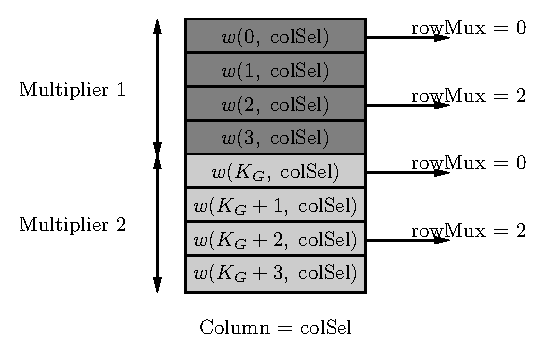
\includegraphics[width=2.5in]{figures/mem-array-prod.eps}
    \caption{A column of the matrix that serves as input to the module. The dark shaded part is for the first multiplier, and the light shaded is for the other, in parallel. The rowMux signal addresses the position within each shaded area}.
    \label{fig:mem-arrayprod}
\end{figure}

\begin{figure*}[!t]
    \centering
    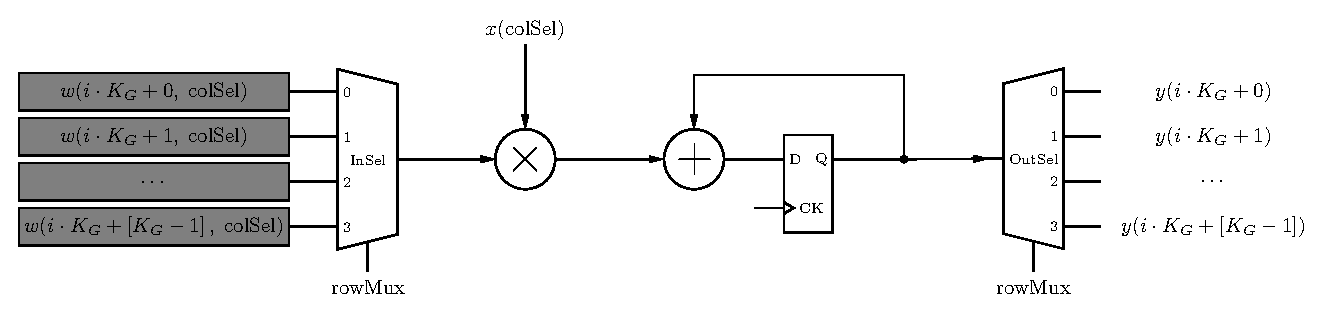
\includegraphics[width=\linewidth]{figures/array-prod.eps}
    \caption{The $i$-th row multiplication unit of the Module, where rowMux and colSel are internal signals produced by the control unit of the module. The flip-flop accumulates the sum, and the output demux selects the appropriate memory position on where to store this value, within the slot attributed to this multiplication, from $i\cdot K_G$ to $i\cdot K_G + \left[K_G-1\right]$}
    \label{fig:array-prod}
\end{figure*}

\subsection{Weight storage}\label{sec:proprarch_ram}
The weights are stored in LUTRAM, and for that purpose, they are declared as a matrix of registers, where the access, both in terms
of write and read operations, is made to each column. The write/read access can be performed simultaneously, since the memory has
separate communication ports for input/output, provided that the \textbf{addresses do not coincide}.

\subsection{Gate Module}\label{sec:proparch_gate}
The Gate modules are responsible for producing the internal signal vectors for $\mb{z}^{(t)}$, $\mb{i}^{(t)}$, $\mb{f}^{(t)}$ and $\mb{o}^{(t)}$. This way,
each Gate module needs to perform three tasks

\begin{enumerate}
    \item Multiply matrix $\mb{W}_*$ by the input vector $\mb{x}^{(t)}$
    \item Multiply matrix $\mb{R}_*$ by the previous layer output vector $\mb{y}^{(t-1)}$
    \item Sum the bias vector $\mb{b}_*$ to the remaining matrix-vector dot product results.
\end{enumerate}
Assuming that the network size $N$ is always larger than the input size $M$, if we use the matrix-vector dot product units of Section~\ref{sec:proprarch_dot}, the multiplication
in task 1 takes approximately $K_G\cdot M$ cycles and the one in task 2 takes $K_G\cdot N$ cycles. This way, tasks 1 and 2 can be performed in parallel, and we can use the extra
time that task 2 takes, relative to task 1,  to perform task 3, and sum the bias vector to the output of task 1, whose result is ready by that time. The module is triggered by a
\verb+beginCalc+ input signal that activates the internal state machine, and outputs a \verb+dataReady+ signal that informs the network that the calculations have been concluded. 
Taking into account the internal state-machine and that the internal datapath is pipelined, the exact number
of clock cycles this module takes to produce an output is $6+K_G\cdot N$.

\begin{figure}
    \centering
    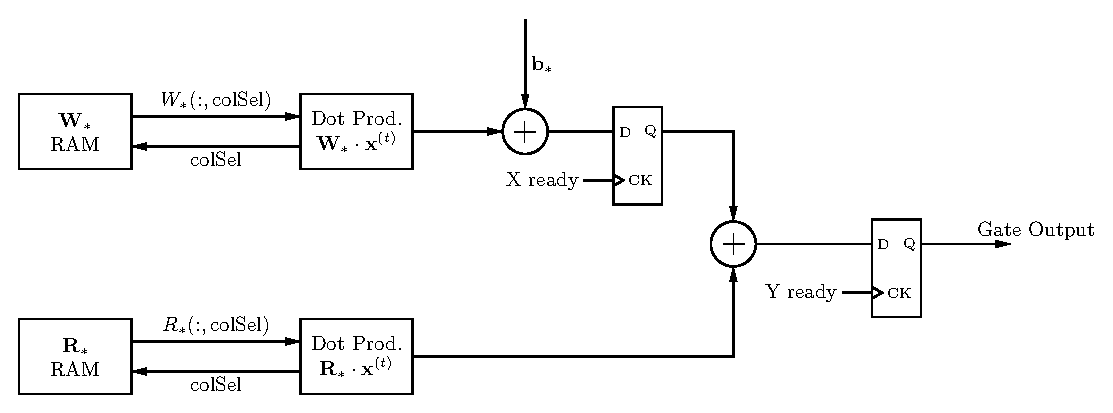
\includegraphics[width=2.5in]{figures/gate.eps}
    \caption[Diagram of the hardware block that implements the Gate]{Diagram of the hardware block that implements the Gate}
    \label{fig:gate}
\end{figure}

\subsection{Network Architecture}\label{sec:proprarch_net}
Equations~\ref{eq:equationsLSTM} suggest that the signals $\mb{z}^{(t)}$, $\mb{i}^{(t)}$, $\mb{f}^{(t)}$ and $\mb{o}^{(t)}$ do not depend on each other -- they
operate only on the current input vector $\mb{x}^{(t)}$ and the previous layer output $\mb{y}^{(t-1)}$ -- and therefore can be calculated in parallel. For that, we
need four Gate Modules working in parallel, each one with its respective weight RAMs for $\mb{W}_*$ and $\mb{R}_*$, and followed by the respective activation
function calculator (detailed in Section~\ref{sec:proprarch_af}). There are three elementwise multiplications, two for producing signal $\mb{c}^{(t)}$ (which
can be done in parallel and then summed elementwise) and one for $\mb{y}^{(t)}$ (which can be done only after applying the activation function $\mb{c}^{(t)}$).

Furthermore, we can avoid a naive translation of the Equations~\ref{eq:equationsLSTM}, which would replicate unnecessary resources (such as elementwise multipliers
and activation function calculators) and require more area to save a negligible number of clock cycles, by noting that one of the operands is the output
of a $\tanh(\mb{x})$ block and the other of a $\sigma(\mb{x})$, and they are then multiplied, elementwise, together. Instead of replicating
these `$\tanh$-$\sigma$-$(\cdot)$wise' structures, we use a \emph{single one} and choose the operand according to the state that the network is currently in. The
issue about the elementwise multiplier for $\mb{c}^{(t)}$, which does not use the $\tanh$ activation function, can be solved by adding another multiplexer that chooses
between the output of the $\tanh(\mb{x})$ module or the signal $\mb{c}^{(t-1)}$. These ideas resulted in the LSTM network design of Figure~\ref{fig:network-opt}, which
is mathematically equivalent to Equations~\ref{eq:equationsLSTM}.

\begin{figure*}
    \centering
    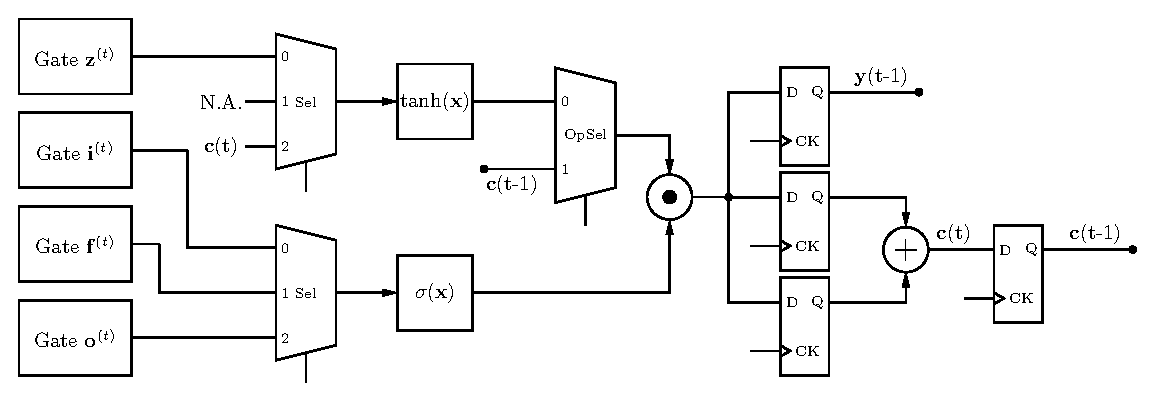
\includegraphics[width=0.9\linewidth]{figures/network-opt.eps}
    \caption[Block diagram of the hardware LSTM Neural Network]{Block diagram of the hardware LSTM Neural Network}
    \label{fig:network-opt}
\end{figure*}
The two left multiplexers control the operands that are fed to the activation function modules, and the selecting signal is generated by the network's state machine,
and its value is incremented after each complete usage of the `$\tanh$-$\sigma$-$(\cdot)$wise' structure: this is where the time multiplexing of the structure takes place.
Since in state $\verb+Sel+=1$ the left operand of the elementwise multiplier (the one that preceded the flip-flops in the previous design) is the signal $\mb{c}^{(t-1)}$,
another multiplexer was added before the elementwise multiplication, to select the $\mb{c}^{(t-1)}$ signal in that particular case, and the output from the $\tanh(\mb{x})$ block, otherwise.

The registers on the right hand side of Figure~\ref{fig:network-opt} are activated by signals generated within the network's state machine that enable the appropriate register, placing the
output from the elementwise multiplier in the correct place. The first activated register is the middle one, which keeps the result from the elementwise mutiplication of the $\mb{z}^{(t)}$
and $\mb{i}^{(t)}$ vectors, then, after a full operation of the `$\tanh$-$\sigma$-$(\cdot)$wise' structure, the bottom register saves the other portion of the sum that evaluates to the $\mb{c}^{(t)}$
signal. Lastly, the top register saves the network output $\mb{y}^{(t)}$, which in the next incoming sample becomes $\mb{y}^{(t-1)}$ and is used by the Gate modules in this next batch of calculations.

Now, since there is only a single elementwise multiplier and only two activation function calculators, the total requirement for DSP slices is simply
\begin{equation}\label{eq:numdsp_network-opt}
    4\frac{2N}{K_G} + 2N + N = N \left( \frac{8}{K_G} + 3 \right),
\end{equation}
where we see that we saved $5N$ multipliers, which for a large value of $N$ can have a decisive impact. In terms of speed performance, although the Gate
calculation time remains the same, now the `$\tanh$-$\sigma$-$(\cdot)$wise' structure runs for 3 consecutive times. After adjustments to the state machine, and accounting for
pipelining and synchronization within the datapath, the number of clock cycles needed after the gate module calculations is 27, so the total clock cycles needed to perform a
complete forward propagation are

\begin{equation}\label{eq:numcc_network-opt}
    (N \cdot K_G + 6) + 27  = 33 + N\cdot K_G
\end{equation}
which is only 13 clock cycles more than a fully-parallel, naïve architecture. For instance, an $N=32$ neuron network would
require 320 DSP slices, while this new architecture uses 160, at the expense of 13 more clock cycles.

\section{Results}\label{sec:results}

\subsection{Validation}\label{sec:res-val}

The functionality of the network was verified against a Python model of an LSTM network that was developed as a reference,
both for the forward propagation of the network, as well as for the training algorithm. Python and Numpy were used rather than MATLAB,
since the former has higher performance for the same level of code complexity. The model was trained using the SPSA method~\cite{Spall98}.

The learning problem presented to both the software and hardware network is the \textbf{addition} of two binary numbers of 8 bits. The $i$-th
bit of each number is fed to the network as a vector, and the network outputs its prediction of the correct value of the $i$-th bit
of the \emph{result}. After the whole number is processed, the memory cells of the LSTM network are reset and a new addition
task can be presented to the network. Even though this seems a rather simple problem, it accounts for all the essential issues at which this
network excels: first, this is a \emph{classification} problem in which the Machine Learning algorithm needs to output a prediction based on
the input feature vector, and that prediction has to take into account the \emph{history} of predictions and inputs so far, because the current
bit is the sum of not only the bits of the two operands, but also the \emph{carry} generated at the last few positions -- this is where the
memory cells of this special Recurrent Neural Network come into effect.

The software network was trained for 50 epochs. In each epoch, 5000 training sequences were presented, and then tested with 100 sequences, where the
prediction error was evaluated for that epoch. The trained weights were loaded into the network and several addition problems
were fed to the Network in the testbench, which yielded no errors.

\subsection{Synthesis}\label{sec:results_synth}
The proposed network was first synthesized for a Xilinx XC7Z020 SoC, for sizes $N \in \left\{4, 8, 16, 32\right\}$, varying the resource sharing parameter $K_G$, while keeping the number of inputs set
to $M=2$. For a network size of 32 and $K_G=8$, the LUT usage exceeded the LUT resources available in the FPGA, so only lower values of $K_G$ were
successfully synthesized. This is because of the complexity of the sharing logic for the multipliers of the Matrix-vector Dot Product Module in~\ref{sec:proprarch_dot}. To synthesize the
design for sizes $N \in \left\{64, 128 \right\}$ a Virtex-7 VC707 board was used, which as a XC7VX485T (speed grade -2) FPGA core.

\subsubsection{Maximum Frequency}\label{sec:results_synth_maxfreq}
The maximum clock frequency that does not cause timing violations of any sort is plotted in Figure~\ref{fig:maxfreq}. For $N=4$, since there are
only 4 rows to be multiplied, the maximum value of $K_G$ is 4, and hence no synthesis was performed for $K_G = 8$ (N.A.); also,
since $K_G = 2$ and $N=32$, a network such as theses would use $32(8/2+3) = 224$ DSP slices, that exceeds the 220 slices
available in the XC7Z020, so there is no synthesis data for that value (N.D.), as well.

It is clear that with increasing $K_G$, the maximum clock speed decreases, and that decrease is steeper for larger values
of $K_G$. This means that there is a critical path in the Matrix-Vector multiplication unit, whose multiplexer becomes
increasingly complex for higher values of $K_G$. On the other hand, when $K_G$ is the same, smaller networks are faster
than larger networks. The fastest design is an $N=4$ and $K_G = 2$ network, with a clock frequency of $158.228$ MHz, and
the slowest one is an $N=32$ and $K_G=4$ network, clocked at $101.523$ MHz. The reference design used for validation in
Section~\ref{sec:res-val} is an $N=8$ and $K_G=2$ network clocked at $154.321$ MHz, which yields a clock period of
\SI{6.48}{\nano\second}. The maximum clock achievable for the VC707 networks is 140.854 MHz, for $N=64$ and $N=128$.

\begin{figure}
    \centering
    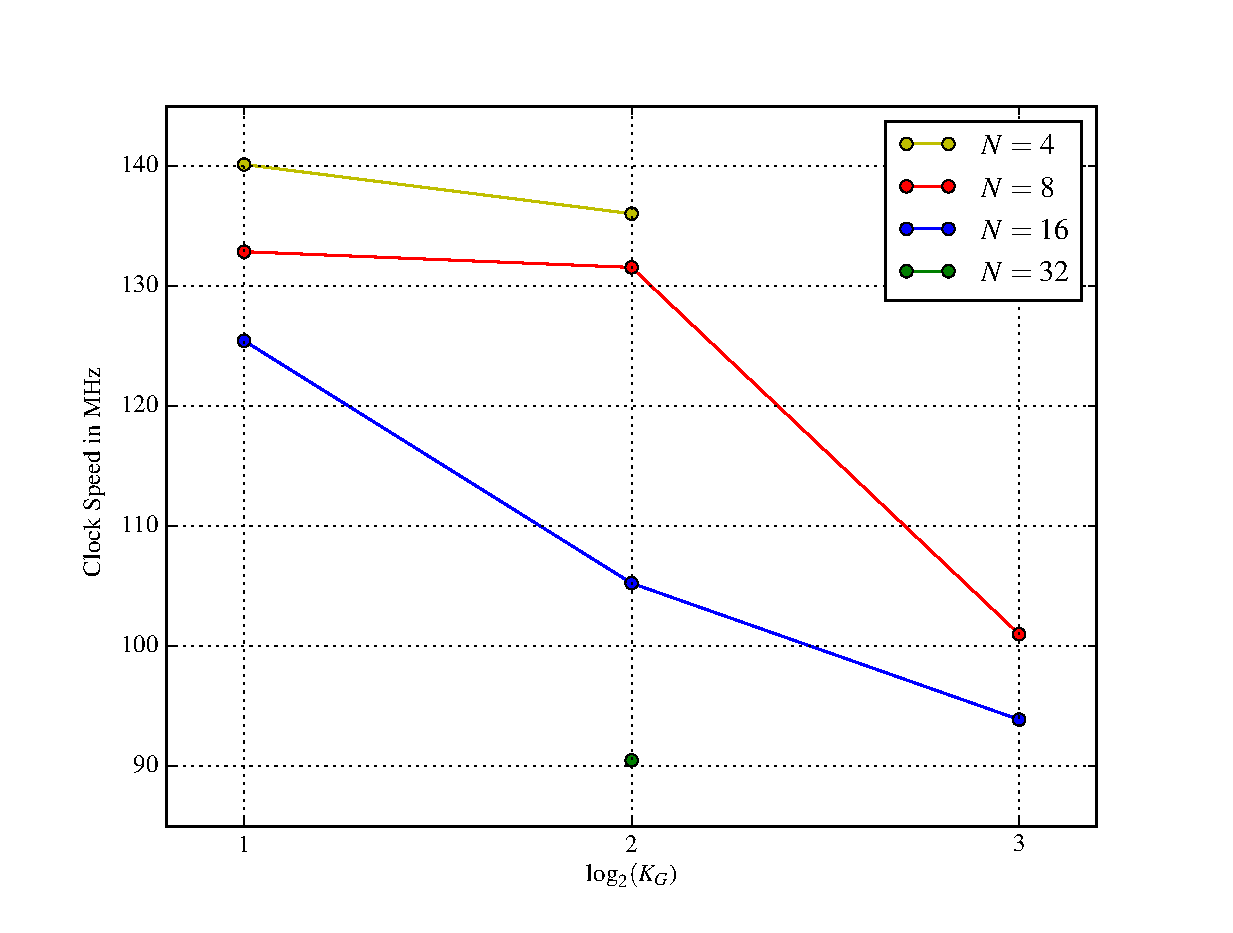
\includegraphics[width=\linewidth]{figures/maxfreq.eps}
    \caption{The maximum achievable clock frequency for feasible network sizes in the XC7Z020}
    \label{fig:maxfreq}
\end{figure}

\subsubsection{DSP Slices Usage}\label{sec:results_synth_dsp}
The estimates made in Equation~\ref{eq:numdsp_network-opt} were shown to be accurate, as Figure~\ref{fig:dspused} confirms.
The reference network design with $N=8$ uses 56 DSP slices, which corresponds to $25.45\%$ of the total number of DSP slices available.

\begin{figure}
    \centering
    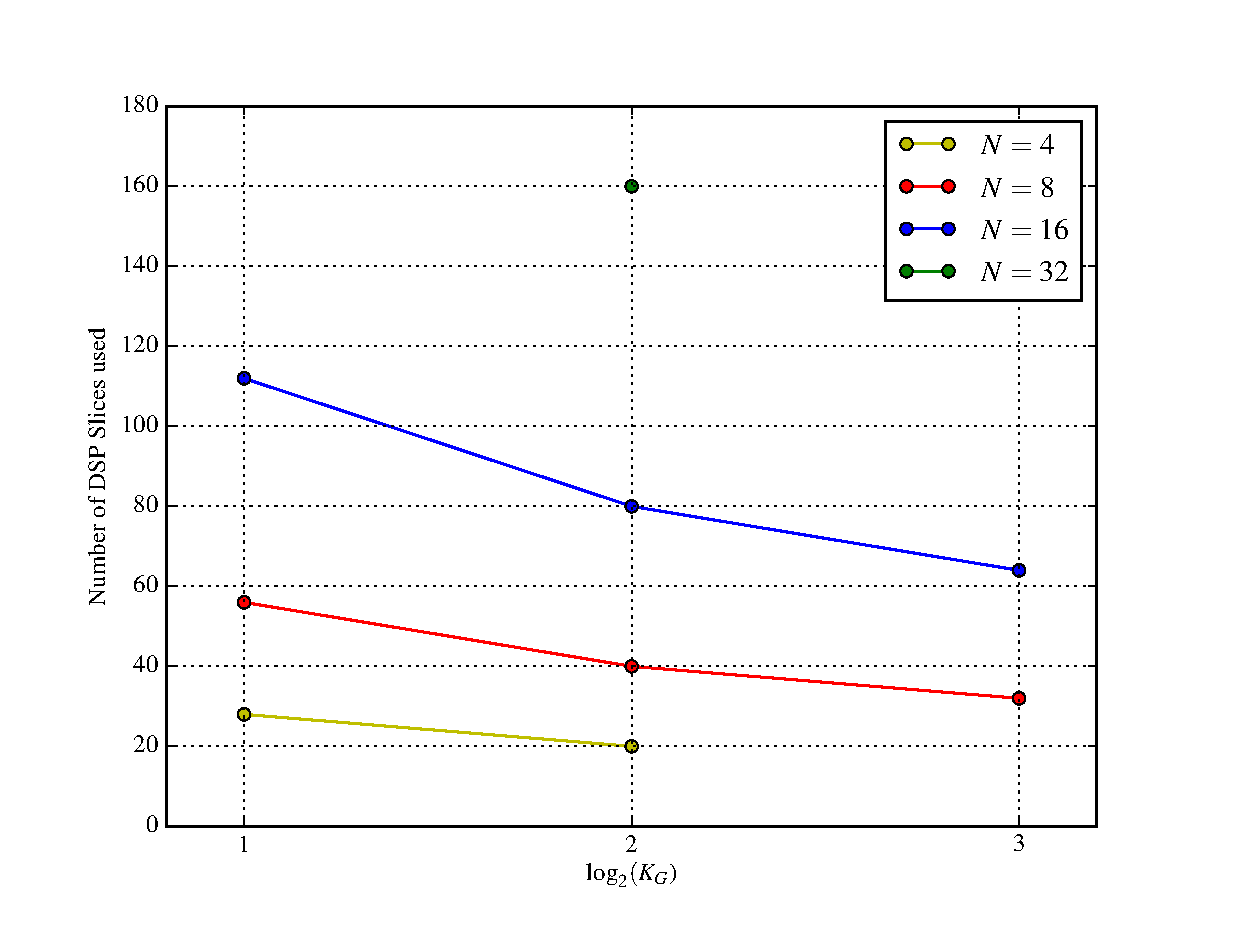
\includegraphics[width=\linewidth]{figures/dspuse.eps}
    \caption{The number of DSP slices used for several Network Sizes $N$ and resource sharing level $K_G$}
    \label{fig:dspused}
\end{figure}
The DSP usage for the VC707 was also accurate.

\subsubsection{Other Resources Usage}\label{sec:res-synth-otheres}
The LUT, LUTRAM and Flip-Flop usages are discussed here. In Table~\ref{tab:lut}, the usage of LUTs is reported. We can see
that although there is not a clear trend on how the LUT usage varies with increasing $K_G$, it is clear, and expectable, that
the LUT usage increases with the size of the network by an approximate factor of 2, from $N=2$ to $N=16$. As for $N=32$, the
usage does not follow this apparent trend, and rises sharply to 91\%. For $K_G = 8$ the usage surpasses the maximum amount
of LUTs available in the XC7Z020.

\begin{table}
	\caption{LUT usage for different $N$ and $K_G$ in the XC7Z020}
	\label{tab:lut}
    \centering
  \begin{tabular}{ | l | c | c | c |}
    \hline
    & $K_G=2$  & $K_G=4$ & $K_G=8$ \\
    \hline
    $N=4$ & 6.87\% & 6.04\% & N.A. \\
    \hline
    $N=8$ & 14.64\% & 13.03\% & 14.11\% \\
    \hline
    $N=16$ & 28.97\% & 27.72\% & 29.85\% \\
    \hline
    $N=32$ & N.A. & 91.09\% & N.D. \\
\hline
  \end{tabular}

\end{table}

As for LUTs, the FF usage also scales according to a $2\times$ factor. In terms of LUTRAM, used to store the network weights,
the amount used increases by 2 with increasing values of $N$, as before, and \textbf{does not} depend on $K_G$. This is because
the amount of weights only depends on the network sizes $M$ and $N$, and not on $K_G$. Furthermore, unlike LUTs, it scales well
with increasing network sizes, and does not pose a limitation on the network size. The usage results for the XC7Z020 are reported in Table~\ref{tab:ff};
the results for the VC707 are in Table~\ref{tab:ff-virtx7}.

\begin{table}
	\caption{Flip-flop and LUTRAM usage for the XC7Z020}
	\label{tab:ff}
    \centering
  \begin{tabular}{ | l | c | c |}
    \hline
         & LUTRAM  & FF  \\
    \hline
    $N=4$ & 0.18\%  & 3.39\% \\
    \hline
    $N=8$ & 4.41\%  & 6.7\% \\
    \hline
    $N=16$ & 8.83\%  & 13.36\% \\
    \hline
    $N=32$ & 17.66\% &  26.45\% \\
\hline
  \end{tabular}

\end{table}


\begin{table}
	\caption{Flip-flop, LUTRAM and LUT usage for the VC707}
	\label{tab:ff-virtx7}
    \centering
  \begin{tabular}{ | l | c | c | c |}
    \hline
         & LUTRAM  & FF & LUT \\
    \hline
    $N=64$ & 24.22\%  & 9.14\% & 24.22\% \\
    \hline
    $N=128$ & 14.09\%  & 18.3\% & 41.82\%\\
\hline
  \end{tabular}
\end{table}

\subsection{Performance}
To evaluate the throughput of the system, a metric was defined based on how many predictions it can produce per second (i.e. produce a new result bit in the output sequence),
in \textbf{millions}. The metric in~\cite{Chang15}, as discussed in Section~\ref{sec:relwork}, is not very informative, since
although a system can perform many calculations per second, if those operations are redundant, that metric has no relevant information
regarding \textbf{how fast} the system can \textbf{perform the actual task it was meant to do}, which in this case is a complete Forward
Propagation through the network. The prediction time is the time elapsed from the moment a new input vector is applied \emph{to} the moment the LSTM
Network produces an output vector. Hence, we multiply the number of clock cycles yielded by Equation~\ref{eq:numcc_network-opt} by the equivalent clock period
from the synthesis clock report of Figure~\ref{fig:maxfreq}. Nevertheless, a comparison on the number of Millions of operations both systems do will be presented further ahead.
This result is reported in Table~\ref{tab:process-time}, where the calculation time of the Python module's Forward Propagation function is
also included. This time was measured using the \textbf{timeit}\footnote{https://docs.python.org/3.5/library/timeit.html}  module, which allows
the evaluation of the execution time of small pieces of code as well as complete functions with arguments. The Python code was run on a Linux System,
powered by an i7-3770k Intel Processor, running at 4.2GHz, with 8GB of RAM.

\begin{table}
	\caption{Total processing time for a single forward propagation on the XC7Z020}
	\label{tab:process-time}
    \centering
    \begin{tabular}{ | l | c | c | c | c | c | }
    \hline
    & $K_G=8$  & $K_G=4$ & $K_G=2$ & Python & Speed-up \\
    \hline
    $N=4$ & N.A.  & 309.68 ns  & 259.12 ns & 65 $\mu$s & $\times251$ \\
    \hline
    $N=8$ & 793.46 ns  & 421.12 ns  &  317.52 ns & 72 $\mu$s & $\times228$ \\
    \hline
    $N=16$ & 1.497 $\mu$s  & 738.19 ns  & 461.336 ns & 96 $\mu$s & $\times208$ \\
    \hline
    $N=32$ & N.D.          & 1.586 $\mu$s & N.A.       & 185 $\mu$s  &  $\times117$ \\
		\hline
  \end{tabular}
\end{table}
The performance increase is impressive, even for the slowest of the designs (the $N=32$ network). The hardware network is, at best, $\times251$ faster than the software counterpart,
and at worst $\times117$ faster. Also, it is noticeable that increasing the level of resource sharing increases the computation time, since the level of parallelism is lower.

To know how many forward propagations we can perform \emph{per second},
we only need to invert the previous values. These values are presented in Figure~\ref{fig:Mclass-psec}. While the $N=8$ and $K_G=2$ network is able to
perform around 3.15 million predictions per second, the Python model can only output around 14 thousand predictions, which is a very significant result that
proves the relevance of this implementation.

\begin{figure}
    \centering
    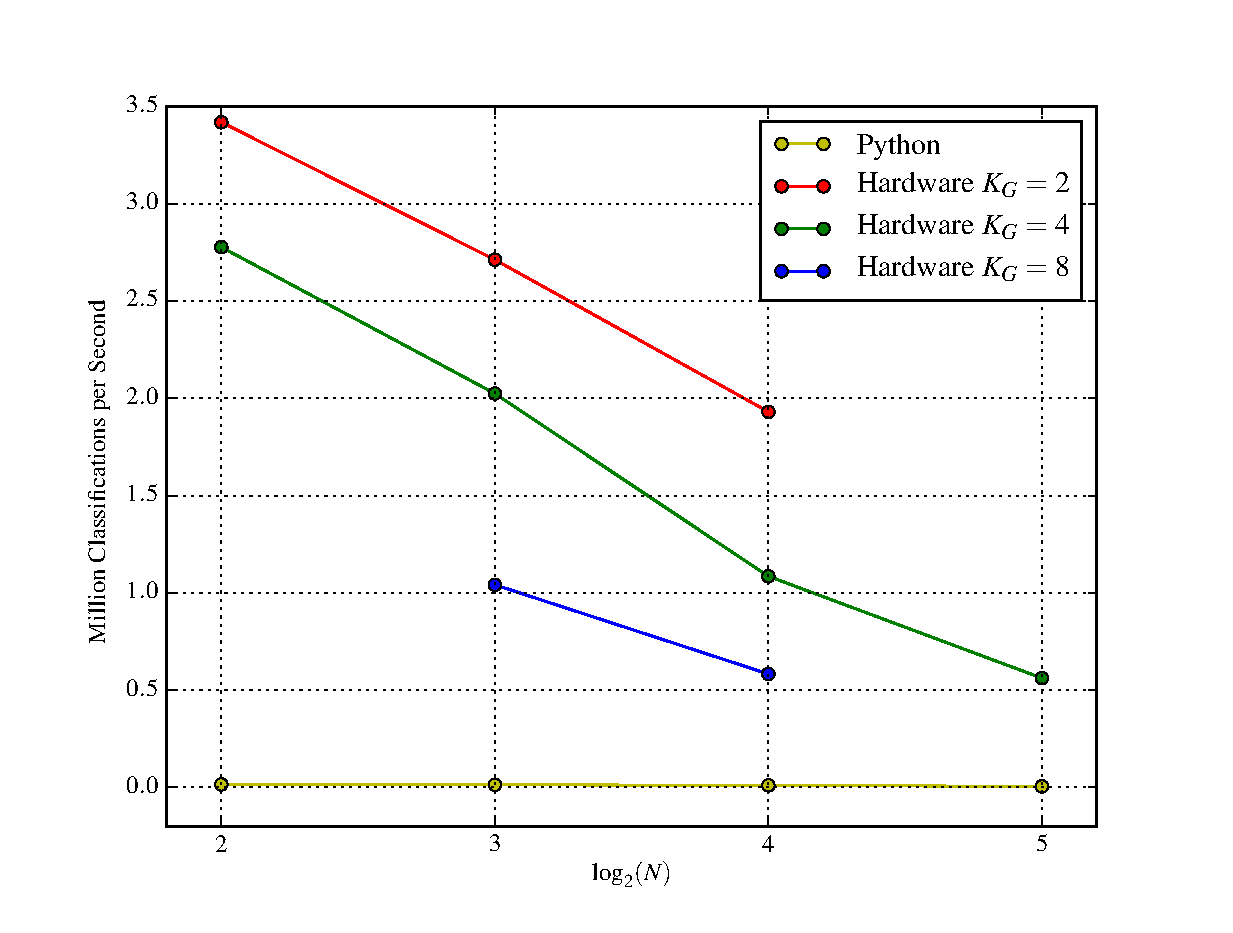
\includegraphics[width=\linewidth]{figures/Mclass-psec.eps}
    \caption[Millions of classifications per second of each design according to the network size $N$]{Millions of classifications per second of each design according to the network size $N$. The comparison is between the software Python model and 3 networks of different levels of resource sharing $K_G$.}
    \label{fig:Mclass-psec}
\end{figure}

As for the larger-sized networks synthesized in the VC707, the results are also very promising. For network sizes of $N=64$ and $N=128$, a complete
forward propagation takes 1.14 $\mu$s and 2.052 $\mu$s respectively, and for both the maximum clock frequency achievable was 140.845 MHz. Since the
design~\cite{Chang15}, for $N=128$, takes an estimated \SI{29.13}{\micro\second} (see Section~\ref{sec:relwork}), our design yields an improvement of $14\times$
over it.
In terms of millions of operations per second (Mops), for an $N=128$ network as the one of~\cite{Chang15}, our work achieves \num{4534.8} Mops per second
while theirs only achieves \num{264.4} Mops per second. This is because, as stated in~\cite{Chang15}, a network of this size performs \num{132.1d3} Mops, and since
our work outputs a sample every $1 \over \SI{29.13}{\micro\second}$, we have that 4534.8 Mops per sec. $=\frac{\num{132.1d3} \; \text{Mops}}{\SI{29.13}{\micro\second}}$.


\subsubsection{Power Consumption}\label{sec:res-synth-power}
Another important metric of the performance of a design is its \textbf{power consumption}. These power consumption estimates are post Place\&Route, and
have a \textbf{medium} confidence level. All  XC7Z020 designs yielded a constant baseline value for the \emph{static} power consumption of around 120 mW,
and the power consumption reported
in Figure~\ref{fig:power} refers to the \emph{total} power consumptions, i.e. both the baseline static power and the dynamic power consumption.
It is clear that the smaller the network is, the less power is consumed, as one would expect. Furthermore, an increasing
level of resource sharing yields a substantially lower power consumption figure: this is because less DSP slices are used as $K_G$ increases.
Of course, even though the power consumption is lower in that case, that comes at the expense of a lower clock frequency and more clock cycles
elapsed per forward propagation.

\begin{figure}
    \centering
    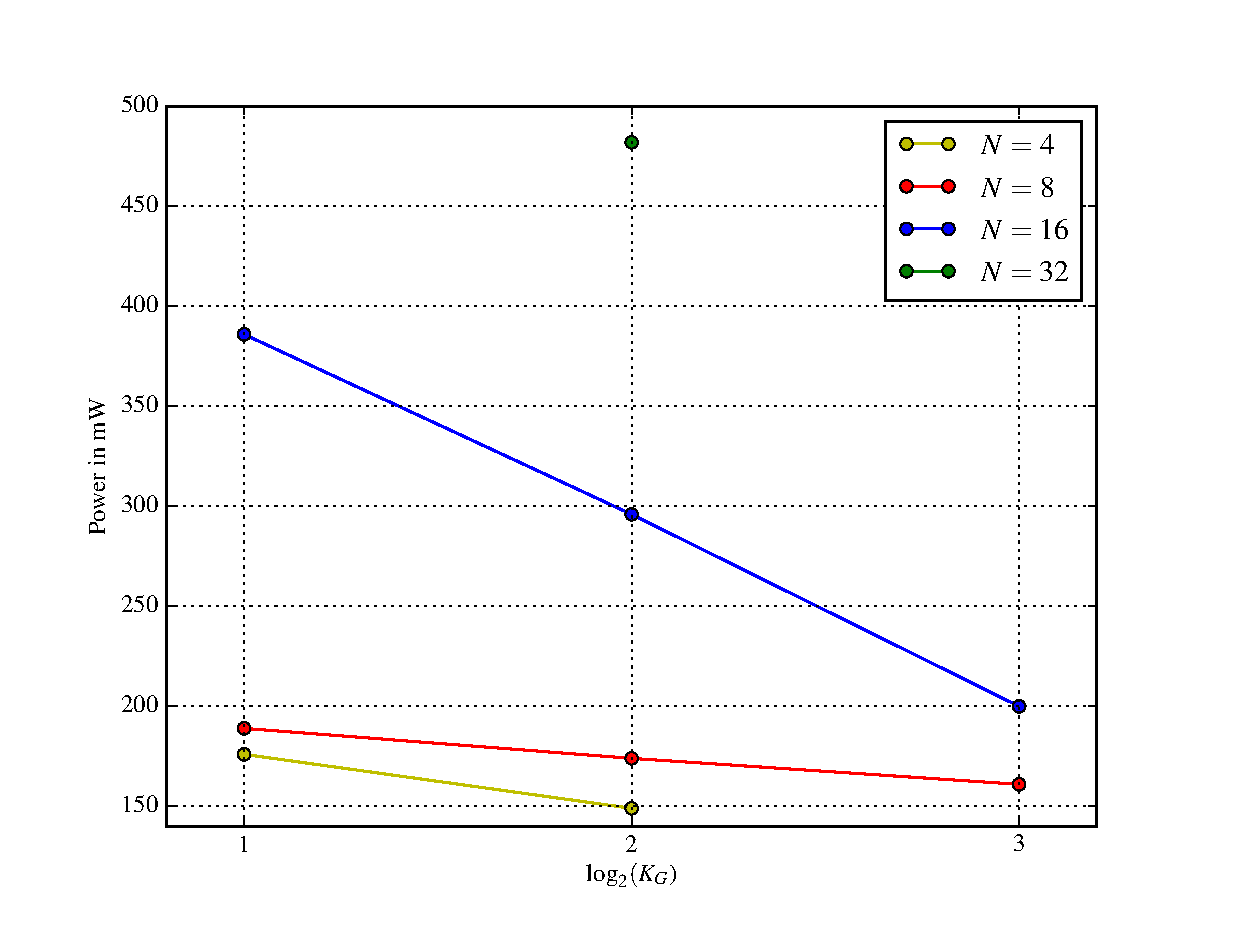
\includegraphics[width=\linewidth]{figures/power.eps}
    \caption{Power Consumption estimates for several Network Sizes $N$ and resource sharing level $K_G$}
    \label{fig:power}
\end{figure}

For the networks synthesized on the VC707, the power consumption was 1.34 Watt for $N=64$, and 1.51 Watt for $N=128$. Since the network size is larger, the power consumption is higher than before, but still within reasonable levels given the complexity of the system. These estimates were provided by Vivado, and have a \textbf{medium} confidence level.

\section{Conclusion}\label{sec:concl}
The LSTM Hardware architecture presented surpassed the performance of the custom-built software implementation by $251\times$, at best,
and also the only current hardware implementation by $14\times$, and solely making use of internal FPGA
resources, achieving a higher level of parallelism. The higher levels of parallelism of this work are achieved at the cost of increasing
design complexity, which limits its scalability to higher sized networks, unlike the implementation of Chang et al.~\cite{Chang15}.
On the other hand, the HDL description of this work is parameterized, and is thus very flexible for networks of any size, not requiring
a redesign of the system every time a differently sized network is required. Furthermore, making use of internal memory makes it suitable
for including an on-chip learning system that can perform training on the network weights.

Given these results, this architecture advances the current state of the art in LSTM Neural Networks
hardware implementations, providing the most efficient implementation to date.

\section*{Acknowledgements}
This work is financed by the ERDF – European Regional Development Fund through the Operational Programme for Competitiveness and Internationalisation - COMPETE 2020 Programme within project \guillemotleft POCI-01-0145-FEDER-006961\guillemotright, and by National Funds through the FCT – Fundação para a Ciência e a Tecnologia (Portuguese Foundation for Science and Technology) as part of project \guillemotleft UID/EEA/50014/2013\guillemotright.


\bibliographystyle{IEEEtran}
\bibliography{bibliography}

\end{document}
